\documentclass{article}
\usepackage{tikz}
\usetikzlibrary{shapes,snakes,calendar,matrix,backgrounds,folding}
\usepackage{verbatim}

\begin{comment}
:Title: PGF version 1.18
:Tags: PGF 1.18, Manual
:Grid: 2x3

A new version of PGF, version 1.18, was recently released. As always with a new release, there are
many new and exciting features and improvements. Below I have summarized some of the new features.
For a full list of changes see the changelog_.


Math library
------------

Mark Wibrow has contributed an impressive and flexible math library. The new
library allows you to use mathematical expression when specifying coordinates.
Example:

.. sourcecode:: latex

    \node at (2*0.5,{2*sin(10)}) {$\gamma$};
    \draw (0,0) -- (pi/4r:1);

A consequence of the new library is that you now can use fractional values
when specifying angular coordinates! You can also plot simple functions inline without
using gnuplot.

Matrices
--------

A TikZ matrix is a new and powerful way of arranging elements of your illustration
in a grid like fashion. It is similar to LaTeX' ``array`` environment and PSTricks'
``psmatrix`` environment. Example:

.. sourcecode:: latex

    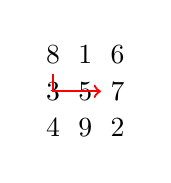
\begin{tikzpicture}
        \matrix (magic) [matrix of nodes]
        {
            8 & 1 & 6 \\
            3 & 5 & 7 \\
            4 & 9 & 2 \\
        };
        \draw[thick,red,->] (magic-1-1) |- (magic-2-3);
    \end{tikzpicture}


Graphic externalization commands
--------------------------------

A common problem when distributing TeX-documents with PGF and TikZ code,
is that colleagues and editors does not PGF installed. New in this version
are a set of commands for creating a version of your document which does not
need PGF installed to compile. Your illustrations are instead created as external
files and included in your document. This can also be useful for illustrations
that are very time consuming to draw.

New node shapes
---------------

Mark Wibrow has contributed two new and highly configurable node shapes:

- ``regular polygon``. The number of sides can be set with the option ``regular polygon sides``.
- ``star``. You can set the number of points with the ``star points`` option.

See the `node shapes`_ example for more information. A few new shapes are also available in the CVS version.

.. _node shapes: /pgftikzexamples/node-shapes/

Calendar library
----------------

With the ``\calendar`` command from the calendar library you can typeset all kinds of calendars.
The library also includes utilities for marking special days and to do various date calculations.

Final words
-----------

I have now briefly described most the new features of PGF 1.18. You should read the manual
carefully to get all the details. The final new feature I will
mention is the paper folding library. Very useful when you want to fold a paper dodecahedron.

PGF and TikZ is getting better and better for each version. Judging from the activity on
various mailing lists and forums, it also seems that the number of users is steadily increasing.


:Source: The PGF and TikZ manual

.. _changelog: ftp://cam.ctan.org/tex-archive/graphics/pgf/doc/generic/pgf/ChangeLog


\end{comment}



\begin{document}

\pagestyle{empty}



% Math engine
\pgfmathsetseed{1}
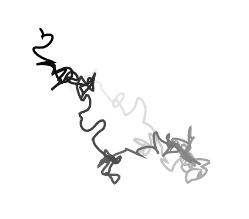
\begin{tikzpicture}[x=5pt,y=5pt,thick,baseline,cap=round]
    \coordinate (current point) at (0,0);
    \coordinate (old velocity) at (0,0);
    \coordinate (new velocity) at (rand,rand);
    \foreach \i in {0,1,...,100}
    {
        \draw[black!\i] (current point)
        .. controls ++([scale=-1]old velocity) and
            ++(new velocity) .. ++(rand,rand)
            coordinate (current point);
        \coordinate (old velocity) at (new velocity);
        \coordinate (new velocity) at (rand,rand);
    };
\end{tikzpicture}

% Inline plotting
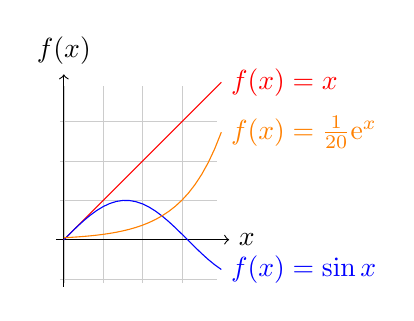
\begin{tikzpicture}[domain=0:4,scale=0.5]
    \draw[very thin,color=black!20] (-0.1,-1.1) grid (3.9,3.9);
    \draw[->] (-0.2,0) -- (4.2,0) node[right] {$x$};
    \draw[->] (0,-1.2) -- (0,4.2) node[above] {$f(x)$};
    \draw[color=red] plot (\x,\x) node[right] {$f(x) =x$};
    \draw[color=blue] plot (\x,{sin(\x r)}) node[right] {$f(x) = \sin x$};
    \draw[color=orange] plot (\x,{0.05*exp(\x)})
        node[right] {$f(x) = \frac{1}{20} \mathrm e^x$};
\end{tikzpicture}

% New node shapes
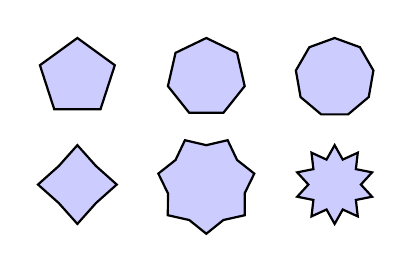
\begin{tikzpicture}
    \matrix[nodes={draw, thick, fill=blue!20,minimum size=1cm},
        row sep=0.3cm,column sep=0.5cm] {
    \node[regular polygon,regular polygon sides=5] {};&
    \node[regular polygon,regular polygon sides=7] {};&
    \node[regular polygon,regular polygon sides=9] {};\\
    \node[star,star points=4] {};&
    \node[star,star points=7,star point ratio=0.8] {};&
    \node[star,star points=10] {};\\
    };
\end{tikzpicture}

% Calendar library
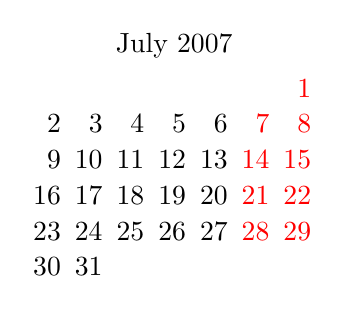
\begin{tikzpicture}
    \calendar [ dates=2007-07-01 to 2007-07-last,
               week list,inner sep=2pt,month label above centered,
               month text=\%mt \%y0
        ]
    if (weekend) [red,nodes={draw=none}];
\end{tikzpicture}


% Matrices
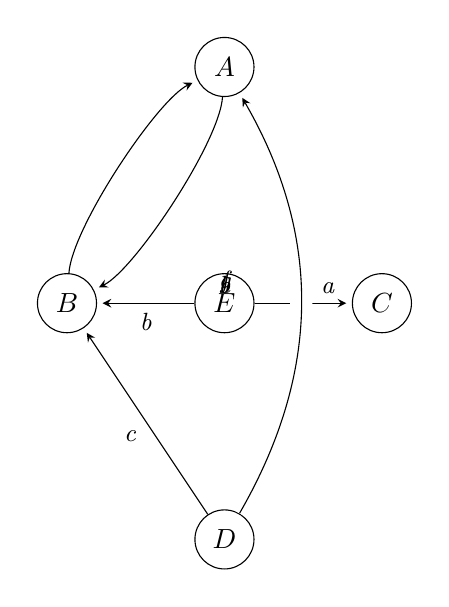
\begin{tikzpicture}[>=stealth,->,shorten >=2pt,looseness=.5,auto]
    \matrix [matrix of math nodes,
        column sep={2cm,between origins},
        row sep={3cm,between origins},
        nodes={circle, draw, minimum size=7.5mm}]
        {
            & |(A)| A & \\
            |(B)| B & |(E)| E & |(C)| C \\
            & |(D)| D \\
        };
    \tikzstyle{every node}=[font=\small\itshape]
    \draw (A) to [bend left] (B) node [midway] {g};
    \draw (B) to [bend left] (A) node [midway] {f};
    \draw (D) -- (B) node [midway] {c};
    \draw (E) -- (B) node [midway] {b};
    \draw (E) -- (C) node [near end] {a};
    \draw [-,line width=8pt,draw=white]
        (D) to [bend right, looseness=1] (A);
    \draw (D) to [bend right, looseness=1] (A)
        node [near start] {b} node [near end] {e};
\end{tikzpicture}

% Paper folding library
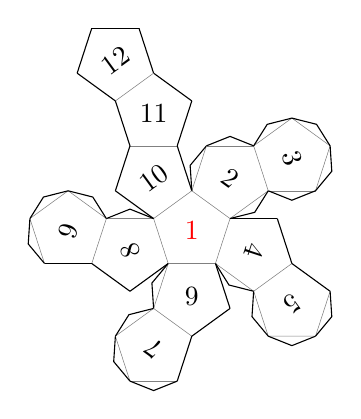
\begin{tikzpicture}[transform shape]
\tikzfoldingdodecahedron
    [folding line length=6mm,
    face 1={ \node[red] {1};},
    face 2={ \node {2};},
    face 3={ \node {3};},
    face 4={ \node {4};},
    face 5={ \node {5};},
    face 6={ \node {6};},
    face 7={ \node {7};},
    face 8={ \node {8};},
    face 9={ \node {9};},
    face 10={\node {10};},
    face 11={\node {11};},
    face 12={\node {12};}];
\end{tikzpicture}

\end{document}

